\chapter{Introduction}
\label{chap:introduction}
\shorttitle{\nameref{chap:introduction}}

This project's motivation is to close the loop between the simulation and the physical world in a robotics application and allow an effortless algorithm transfer from a robot to a robot in general.
The project aims to utilize \ac{ros2}, the second iteration of a popular robotics framework, to develop a standard interface for e-puck2 physical and simulated robots and many other simulated robots.

\section{Problem Statement}
Robotics simulations have been proven to be a powerful tool for research and development as they are easy to set up, cheap, fast, and convenient to use \cite{michel_cyberbotics_2004}.
Usually, the final objective is to perform the experiments on real robots.
Therefore, the problem roboticists are facing is a transition from the simulated to the physical world.
The aim is to make this process simpler and faster, effectively minimizing the simulated and physical world gap. 
The solution should be easy to integrate into the simulation and not cause a significant computational overhead for the physical robot.

Another challenge roboticists are facing with is code reuse. 
In the world of diverse hardware solutions for robots, it is hard to create a modular software solution that can be reused for different robots.
For example, navigation, \ac{slam}, and localization are only a few algorithms widely used in mobile robotics, and many mobile robots could reuse that.
The modular software for the robots is also often requested by researchers as of the need to share the created algorithms with the other researchers, and that can be utilized by the other robots \cite{vaughan_really_2007}.
As for the previous challenge, the solution must be easily integrated into the simulation and not cause significant computational overhead.

The researchers that use e-puck2 and Khepera IV robots are facing those two challenges.
In collaboration with researchers from \ac{epfl} and Cyberbotics employees, the solution has to be implemented for the e-puck2 physical and simulated robot.
The solution also has to be scaled to the Khepera IV simulated robot and potentially other simulated robots.

\section{Project Objective}

As described in the previous section, two challenges in robotics have to be tackled in this thesis.
The first is closing the loop between the simulation and the physical world, and the second is software reuse between different robots.


From the software point of view, solving those problems can be addressed by defining a common \ac{api} for the physical and simulated robot.
\ac{ros} is often used as a meta-operating system for this purpose as the \ac{api} can be defined in \ac{ros}.
The newest version of \ac{ros}, \ac{ros2}, includes useful improvements relevant to the project, and it is about to replace the old version completely.
Therefore, the proposed solution is based on developing \ac{ros2} nodes that closely interact with the hardware and the Webots\footnote{Webots is a desktop application, developed at \ac{epfl}, used to simulate robots.
It will be more closely introduced in the following chapter.} simulation - \ac{ros2} driver.
As a result, a user should have a development workflow, as shown in Fig. \ref{fig:introduction:desired_workflow}.  

\begin{figure}[H]
    \centering
    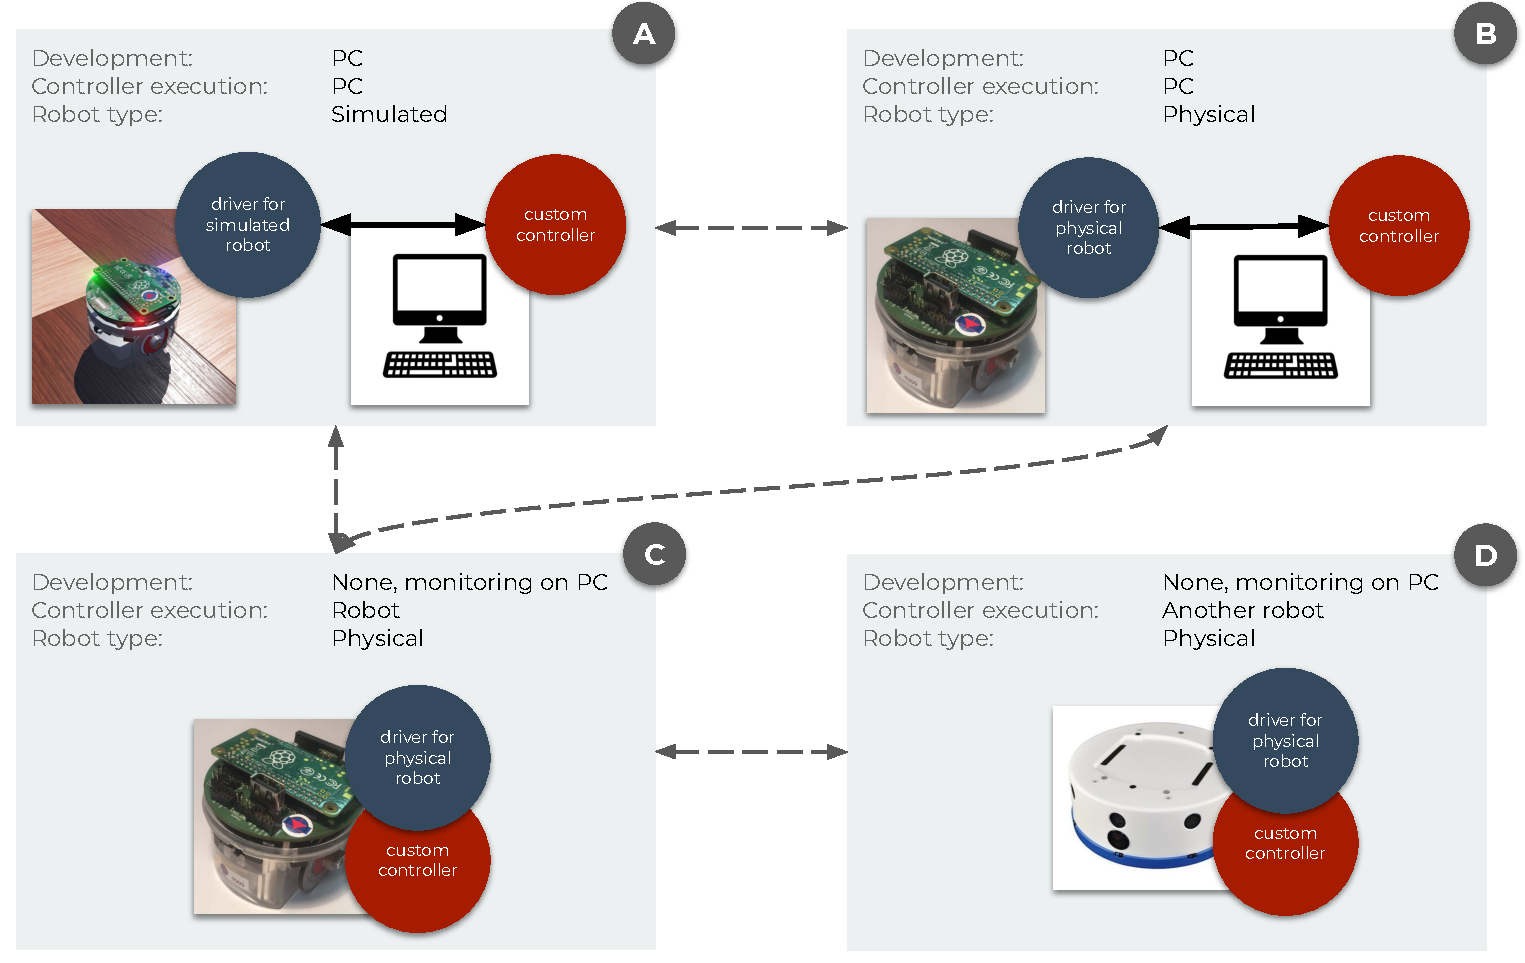
\includegraphics[width=\textwidth]{introduction/figures/desired_workflow.pdf}
    \caption[A development workflow (in robotics) that has to be achieved with the proposed solution]{
        A development workflow (in robotics) that has to be achieved with the proposed solution.
        The circle represents a piece of software that the user wants to develop to control the robot, and it is the same in each scenario.
        The dashed arrows are transitions in the development workflow, while solid the solid arrows represent a network protocol.
    }
    \label{fig:introduction:desired_workflow}
\end{figure}

In Fig. \ref{fig:introduction:desired_workflow} the user develops a robot controller called \texttt{custom controller}.
From the user's perspective, the controller supposed to be the same in each scenario.
First, the user should start by developing the controller on PC and testing it in the simulation.
After the user is satisfied with the robot's behavior in the simulation, the controller can still be executed on the PC, but now it can control the physical robot.
If the robot's behavior is not desired, the user can improve the simulation model and test it again in the simulation, reducing the simulation and the real-world gap.
Once everything works as expected, the user should move the controller to the robot.
Here, it is possible, e.g., to hit the computational limit of the on-board computer, and the controller should be edited and tested again in the simulation, moving back to the on-board computer once it is ready.
Finally, the controller can be shared with the other researchers to evaluate the other robots' control software or further improve it.

The project has to be done in three phases.
First, a specific \ac{ros2} nodes for an e-puck2 simulated and physical robot have to be developed.
Second, examples that utilize the nodes have to be created. 
The purpose of this phase is to evaluate the nodes and to give the users usage examples.
Finally, in the third phase, the specific \ac{ros2} node for e-puck2 simulated robot has to be generalized to support other robots, focusing on Khepera IV and TurtleBot3 robots.
The final software has to be peer-reviewed, united tested, code quality tested, automated with \ac{ci}\footnote{The \ac{ci} automation has to be done with Industrial CI. This \ac{ci} is created by ROS-industrial, an organization committed to close a gap between research and industry by bringing industry standards to \ac{ros2}}, user friendly, and well documented with comprehensive tutorials.

\section{Document Structure}
% Inspired by:
% - https://essay.utwente.nl/59475/1/scriptie_R_van_Domburg.pdf
% - http://www.jedlitschkas.de/downloads/jedlitschka_etAl_reporting.pdf

The structure of the thesis roughly follows the phases described in the previous section.
It should allow readers to skip information, but also to reduce the chance of missing important details.
Therefore, the project is presented as follows:

\begin{itemize}
    \item \textbf{Chapter \ref{chap:background}: \nameref{chap:background}} gives the theoretical background on common concepts, and software and hardware technologies, utilized in the project.
    Also, it clarifies relations with relevant projects.
    
    \item \textbf{Chapter \ref{chap:simulation}: \nameref{chap:simulation}} explains a process used to create a \ac{ros2} node that exposes access to simulated e-puck2 robot's sensors and actuators through \ac{ros2} interface.
    
    \item \textbf{Chapter \ref{chap:physical}: \nameref{chap:physical}} has a goal to explain implementation of the same \ac{ros2} interface for e-puck2 physical robot.
    
    \item \textbf{Chapter \ref{chap:demos}: \nameref{chap:demos}} shows tools, existing packages and custom created controllers that utilize the e-puck2 \ac{ros2} interface.
    
    \item \textbf{Chapter \ref{chap:generalization}: \nameref{chap:generalization}} gives implementation overview on generalized \ac{ros2} driver for simulated robot. It aims to extend e-puck2 driver to support Khepera IV, TurtleBot 3 Burger and potentially the other robots as well.
    
    \item \textbf{Chapter \ref{chap:results}: \nameref{chap:results}} quantifies difference between the \ac{ros2} driver for the simulated and the physical robot, difference between e-puck2 and Khepera IV \ac{ros2} interfaces and it shows simplification resulted by generalization described in the previous chapter.
    
    \item \textbf{Chapter \ref{chap:conclusion}: \nameref{chap:conclusion}} presents the project summary, limitations, impact and potential improvements.
\end{itemize}